% Presentation 4 (July 10): Final Presentation. 
% Focus on Monte Carlo Simulations, Final Results and Shiny App.

% \begin{frame}
%     \frametitle{ }
%     \begin{quote}
%         \centerline{In 30 minutes\ldots}
%         \vskip 16pt
%         \centerline{you'll know how to be financially sophisticated}
%         \centerline{and profit from the financially na\"{i}ve!}
%     \end{quote}
% \end{frame}


\begin{frame}{Outline}
    \tableofcontents
\end{frame}

\section{Recap \& Introduction}

\begin{frame}{Recap}
        \begin{itemize}
            \item {\bf Goal}: Recommend users an optimized credit card portfolio, based on  income/spend and preferences, and study its properties
            \bigskip
            \item Last four weeks we covered: 
            \begin{itemize}
                \item Literature and financially na\"{i}ve/sophisticated behavior
                \item Credit Cards and Budget Data
                \item Algorithm
                \item Sensitivity Analysis
            \end{itemize}
            \bigskip
            \item We found that spending on $\sim$5 cards is the sweet spot for most people, with a minimum Return-On-Spend of $\sim$3.2\% (and max $\sim$6.5\%)
        \end{itemize}
\end{frame} 

\begin{frame}{In this final presentation}
    \begin{itemize}
        \item Some flaws fixed and visualizations improved
        \bigskip
        \item Monte Carlo Simulations
        \begin{itemize}
            \item Setup
            \item Analysis of the results
        \end{itemize}
        \bigskip
        \item Presentation of the Shiny App
        \bigskip
        \item Future work
    \end{itemize}
\end{frame} 

\section{Fixed \& Improved}

% FIXED AND IMPROVED
% - Updated the algorithm so that single-use benefits are no longer double counted
% - Updated the marginal benefit vs number of cards plot for 10 incomes 
% - Improved the portfolio plot to Waterfall plot, so we can see the portfolio and
%   marginal benefits, total benefits, in 1 plot
%

\begin{frame}{Fixed: Single-Use Benefits Stacking}
    \begin{columns}[c]
        \begin{column}{0.7\textwidth}
            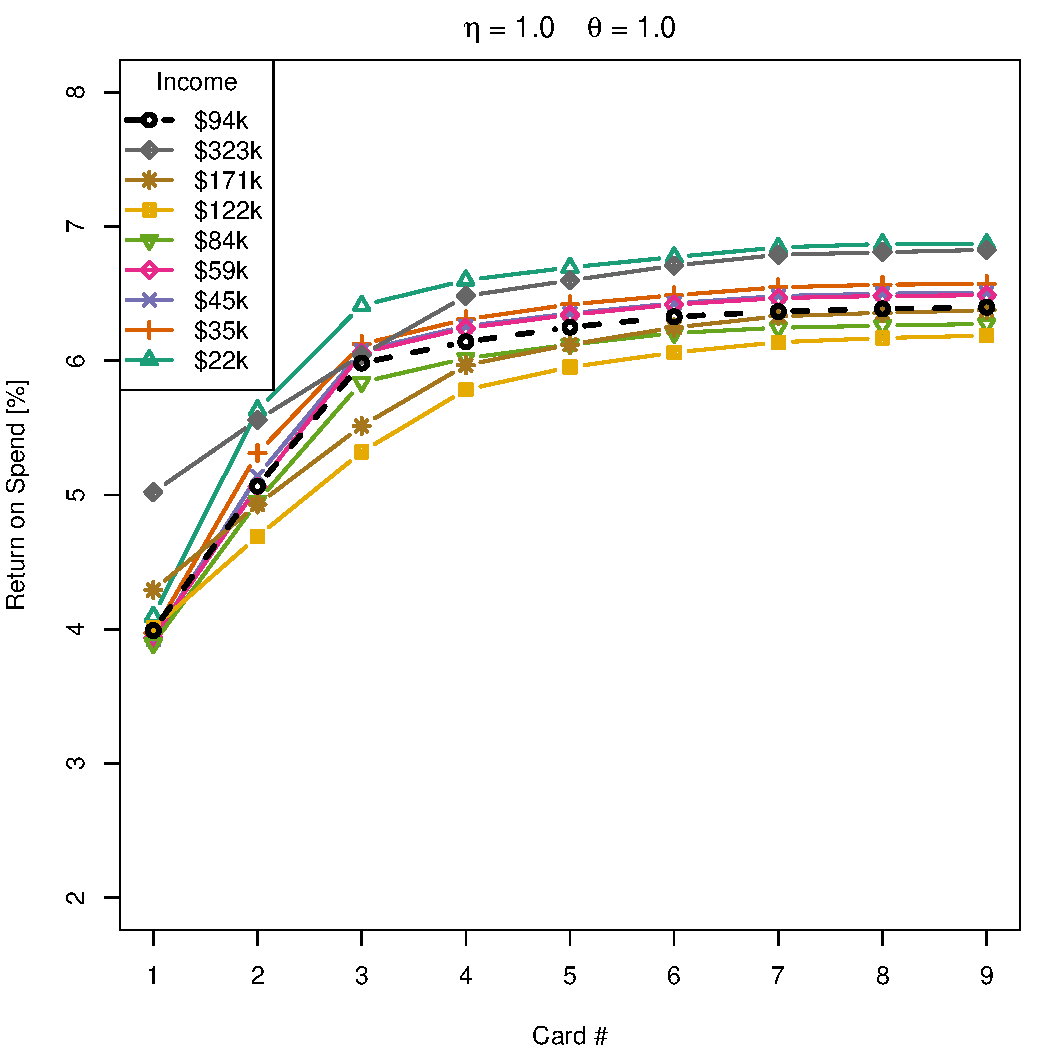
\includegraphics[width=0.9\textheight]{../Figures/ROSvsKvsIncome_1_1.pdf}
        \end{column}
        \begin{column}{0.3\textwidth}
            \centering
            Using a better color scheme, combined with symbols.
            \vskip16pt
            Some benefits are now set to 0 after first selection.
            \vskip16pt
            \emph{Note:} Benefits could still be lucrative for low spenders!
        \end{column}
    \end{columns}
\end{frame} 

\begin{frame}{Unchanged: Number of Cards}
    \begin{columns}[c]
        \begin{column}{0.7\textwidth}
            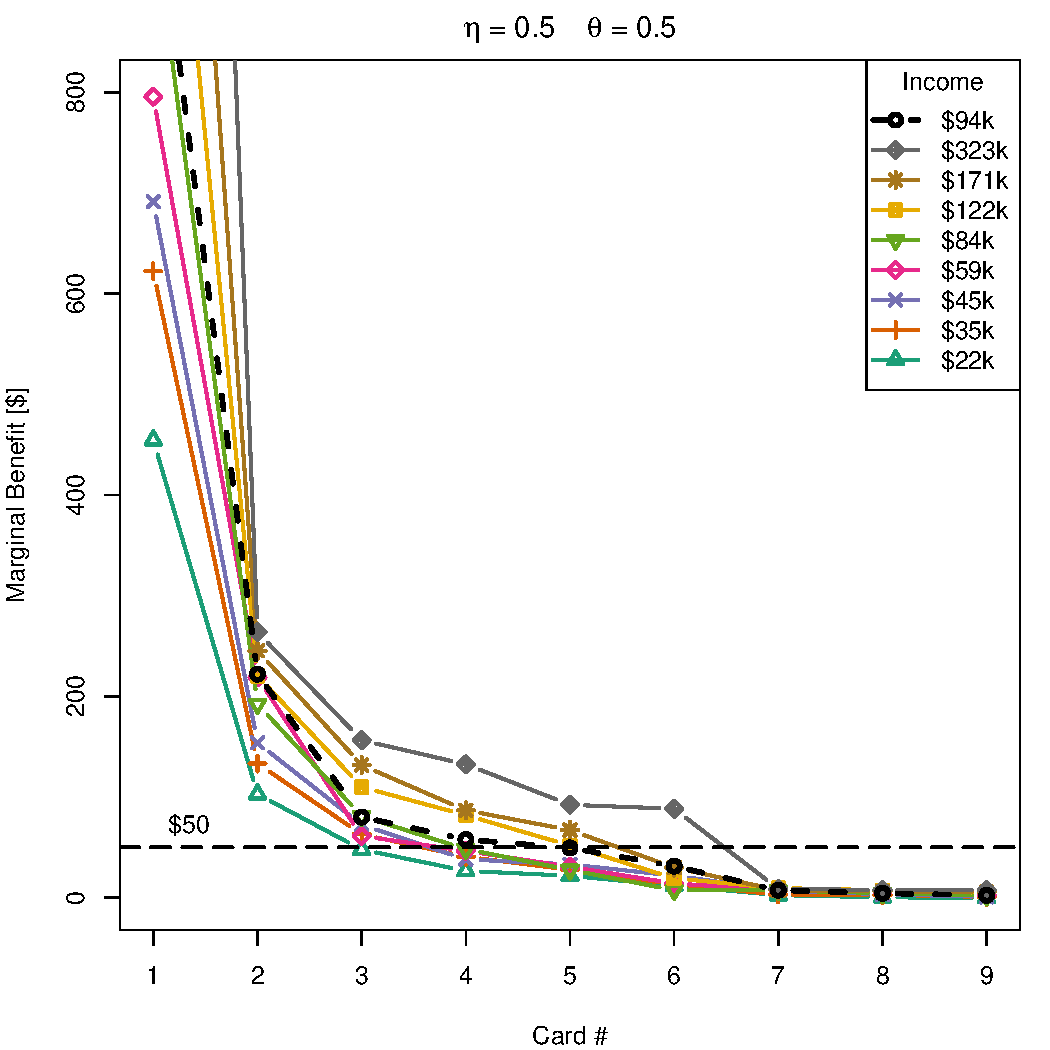
\includegraphics[width=0.9\textheight]{../Figures/MBvsKvsIncome_05_05.pdf}
        \end{column}
        \begin{column}{0.3\textwidth}
            \centering
            % Just to show that this conclusion didn't change after the improvements.
            Four or five cards remains a reasonable choice for most people.
        \end{column}
    \end{columns}
\end{frame} 

\begin{frame}{Improved: Portfolio Visualization}
    \begin{columns}[c]
        \begin{column}{0.7\textwidth}
            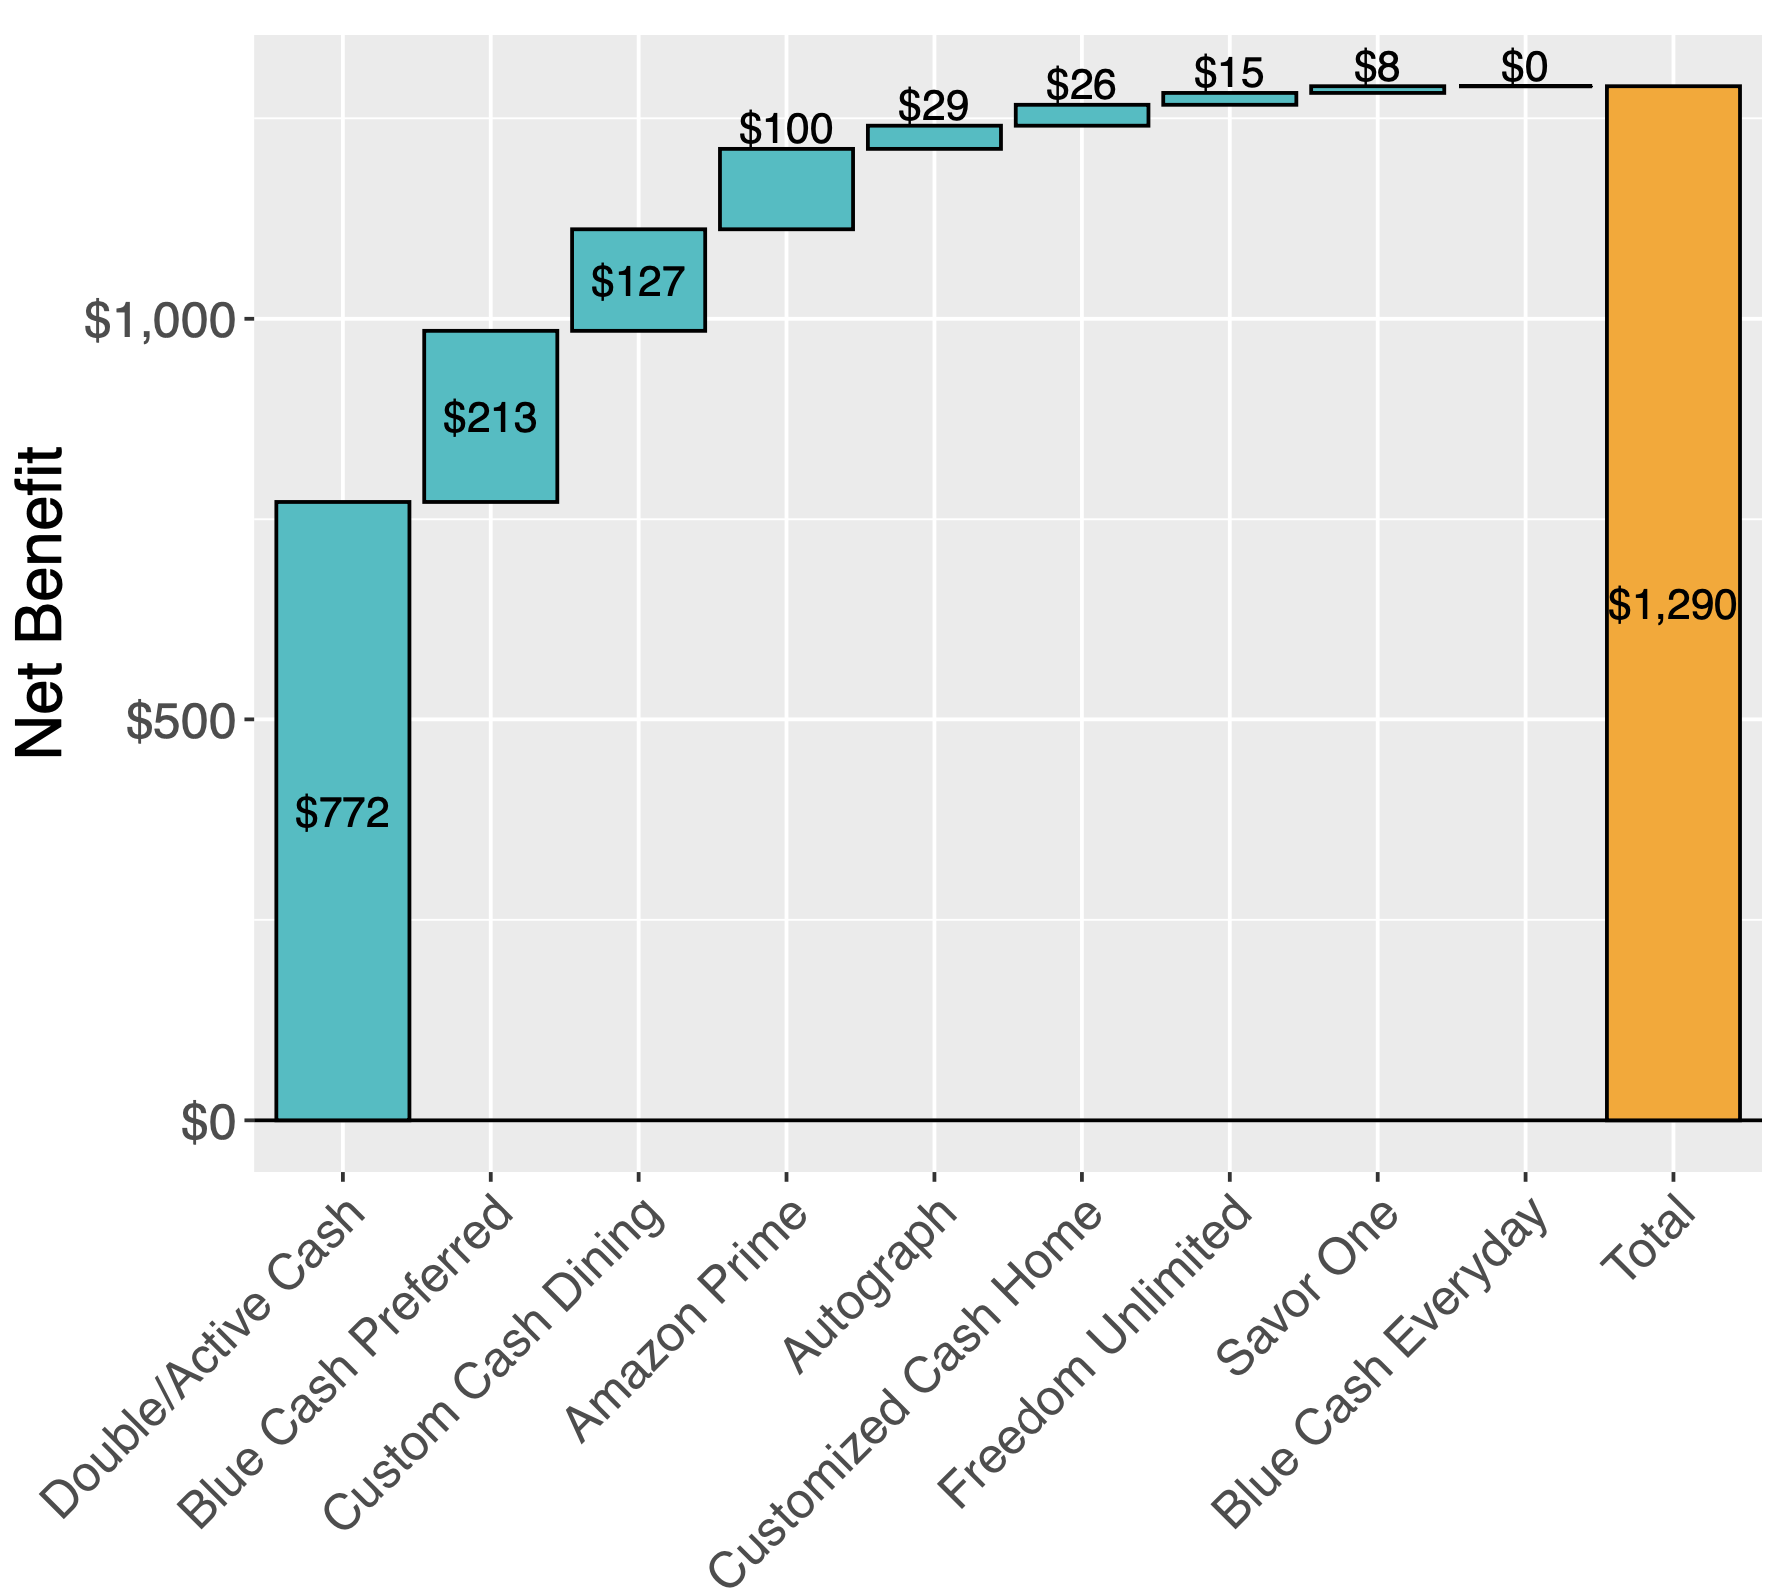
\includegraphics[width=0.9\textheight]{../Misc/Waterfall_avg_9_0_0.png}
        \end{column}
        \begin{column}{0.3\textwidth}
            \centering
            New ``waterfall'' plot to visualize the portfolio (thanks to Jared). 
        \end{column}
    \end{columns}
\end{frame} 


\section{Monte Carlo Simulations}

% MONTE CARLO SIMULATIONS
% - Downloaded Microdata from the ACS Census Data (American Community Survey) for 
%  all 168 Florida counties. 2022 Family Income. FINCP
% - Show IncomeDistribution.pdf with lognormal fit

\begin{frame}{Monte Carlo Simulation Setup}
    \begin{itemize}
        \item By random sampling realistic incomes and preferences, we get a better idea about the average benefits
        \bigskip
        \item Sampled 100,000 times (with replacement):
        \begin{itemize}
            \item 2022 Florida Family Incomes (ACS Census Microdata)
            \item Corresponding budget from BLS CES (9 income bins)
            \item Number of cards: 1--8 (uniform)
            \item Use of Transfer Partners: fraction 0.0--1.0 (uniform)
            \item Use of Benefits: fraction 0.0--1.0 (uniform)
        \end{itemize}
        \bigskip
        \item Sampled 100,000 portfolios, keeping track of Net Benefits, Return on Spend, and (aggregated) count of selected cards (took $\sim$2 hours)
        \item Saved output to \texttt{.csv} files for analysis
    \end{itemize}
\end{frame}

\begin{frame}{Florida Family Income Distribution (observed)}
    \begin{columns}[c]
        \begin{column}{0.7\textwidth}
            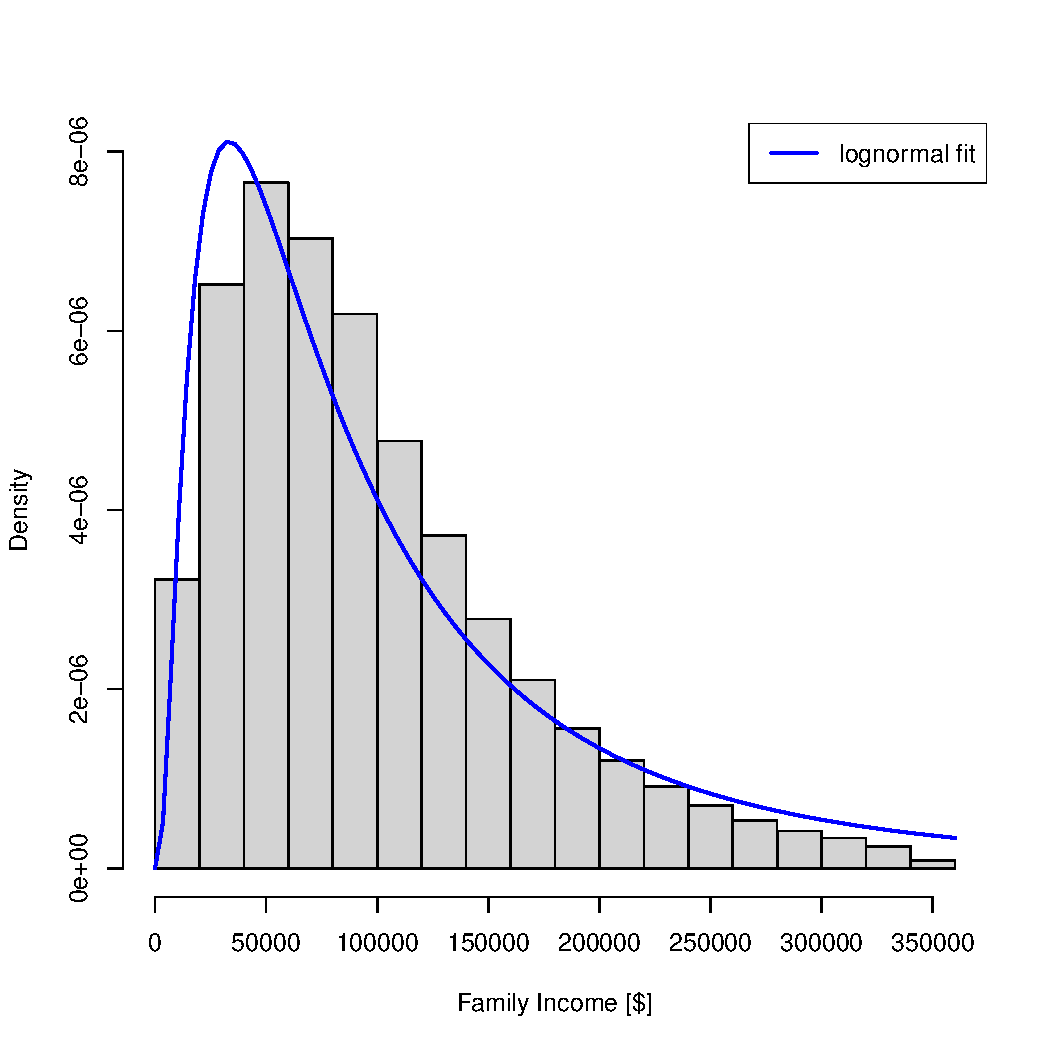
\includegraphics[width=0.9\textheight]{../Figures/IncomeDistribution.pdf}
        \end{column}
        \begin{column}{0.3\textwidth}
            \centering
            57,005 observations (not showing $>$ \$350,000). 
            \vskip16pt
            Mean: \$121,306. Median: \$85,900. 
            \vskip16pt
            Approximates a lognormal distribution.
        \end{column}
    \end{columns}
\end{frame} 

\begin{frame}{Return on Spend Distribution (simulated)}
    \begin{columns}[c]
        \begin{column}{0.7\textwidth}
            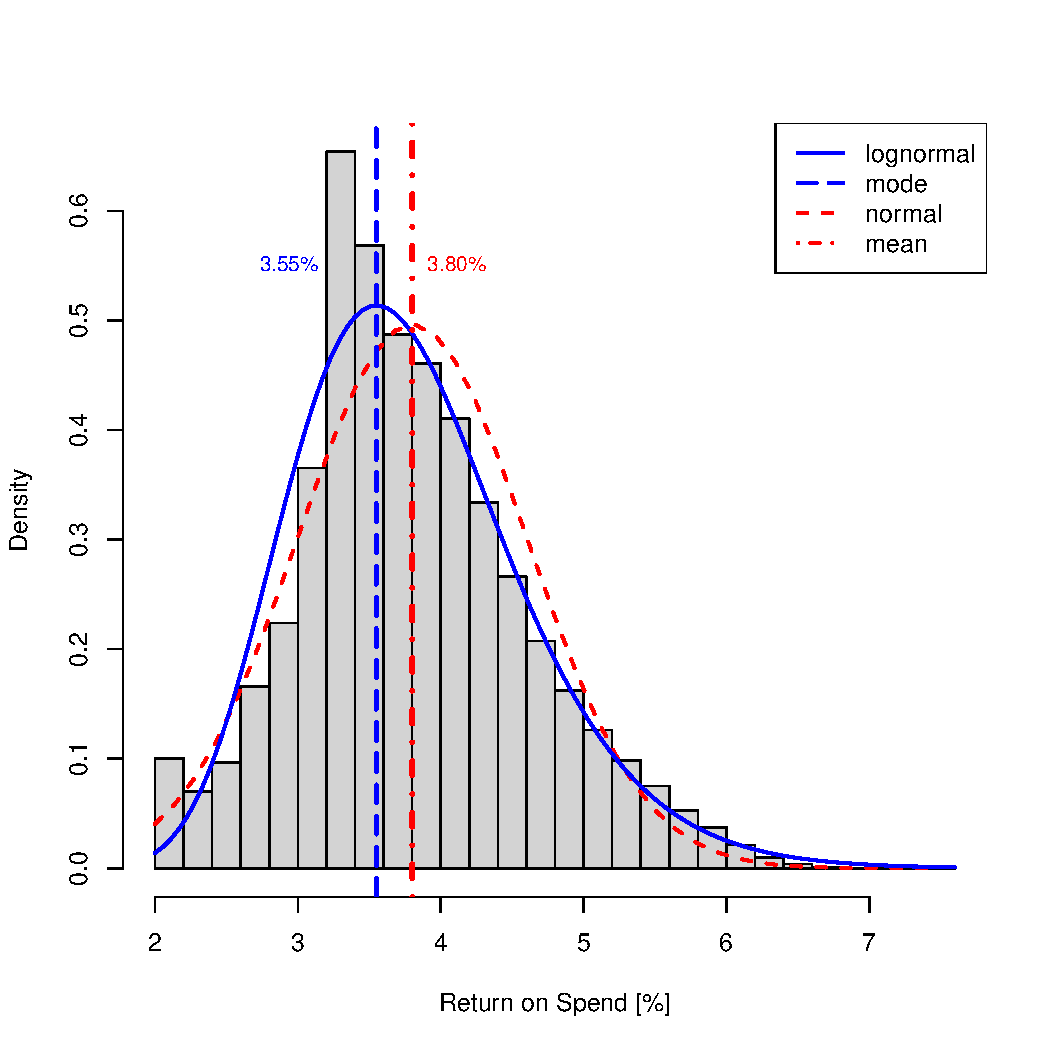
\includegraphics[width=0.9\textheight]{../Figures/MC_ROS_Histogram.pdf}
        \end{column}
        \begin{column}{0.3\textwidth}
            \centering
            Approximates a lognormal distribution. 
            % Standard Deviation of ROS was 0.80
        \end{column}
    \end{columns}
\end{frame} 

\begin{frame}{Smoothed Scatterplot (simulated)}
    \begin{columns}[c]
        \begin{column}{0.7\textwidth}
            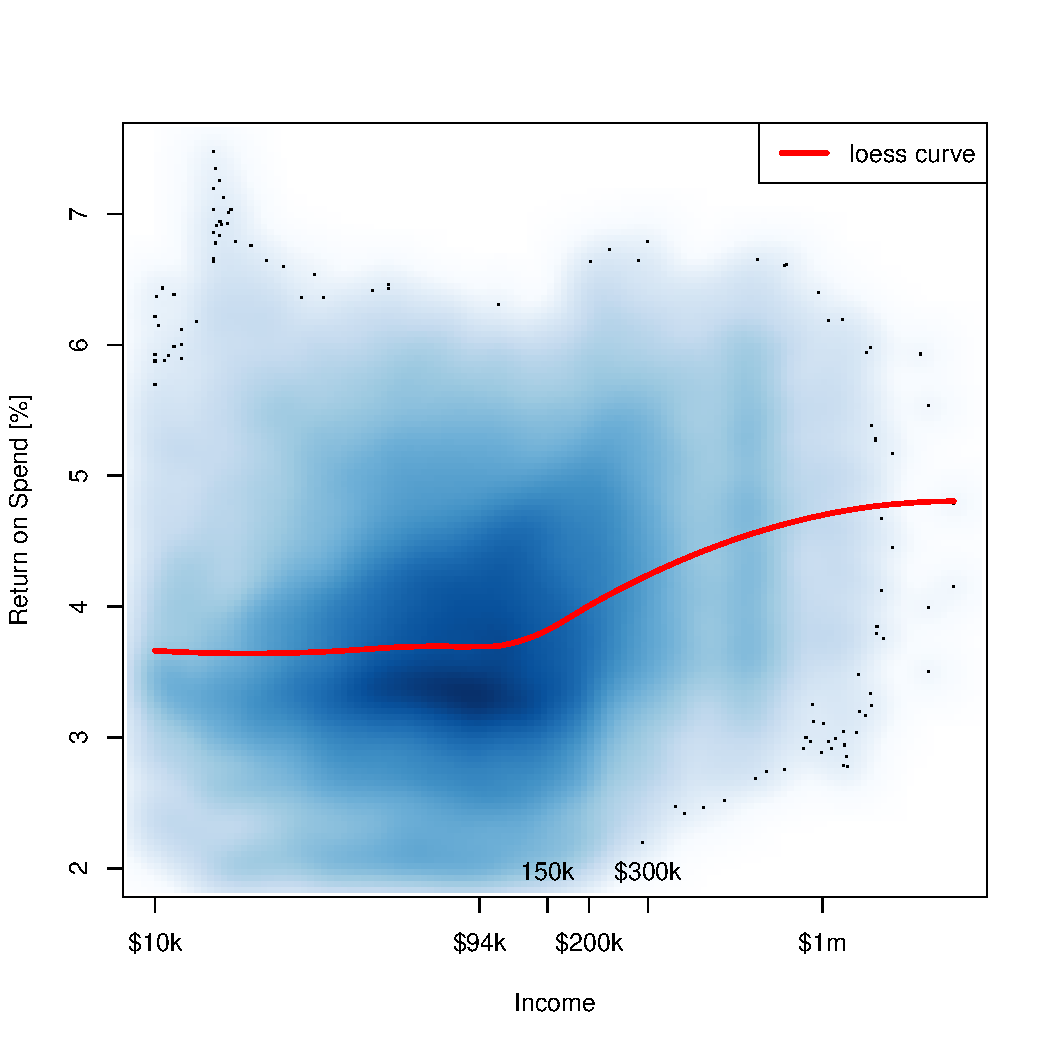
\includegraphics[width=0.9\textheight]{../Figures/MC_ROS_vs_Income.pdf}
        \end{column}
        \begin{column}{0.3\textwidth}
            \centering
            Although spending relatively less of their income, above $\sim$\$100,000 users benefit more from their credit cards.
            \vskip16pt
            (\emph{note the logarithmic x-axis})
        \end{column}
    \end{columns}
\end{frame} 


\begin{frame}{Shifting Spending Patterns (BLS CES data)}
    \begin{columns}[c]
        \begin{column}{0.7\textwidth}
            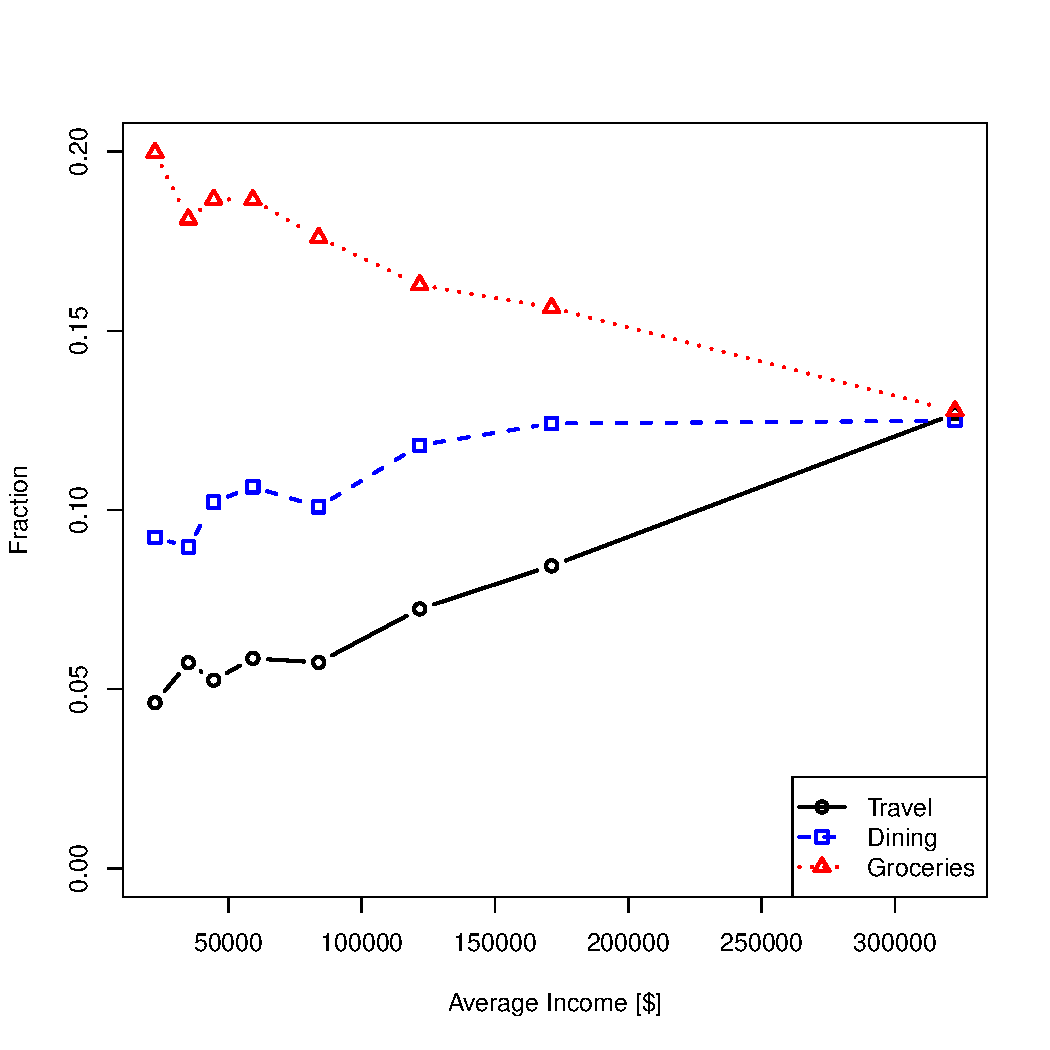
\includegraphics[width=0.9\textheight]{../Figures/TravelDiningFraction.pdf}
        \end{column}
        \begin{column}{0.3\textwidth}
            \centering
            % TravelDiningFraction.pdf  -> shows that after $100,000 especially Travel increases compared to lower incomes, and travel has high multipliers. 
            The best rewards are found on travel categories, rewarding higher incomes disproportionally. 
        \end{column}
    \end{columns}
\end{frame} 

\begin{frame}{Most Recommended Cards}
    \begin{center}
        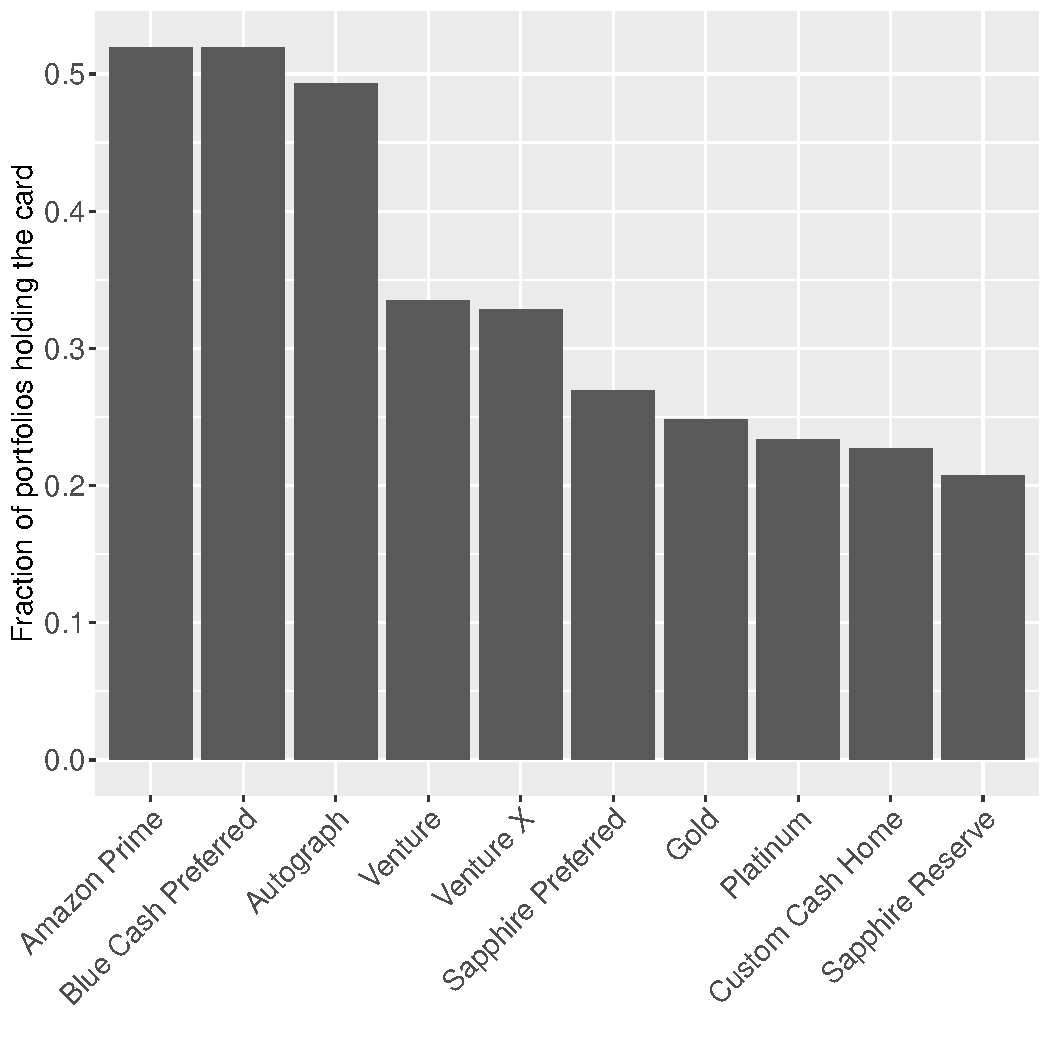
\includegraphics[width=0.9\textheight]{../Figures/MC_Popularity_M100k.pdf}
    \end{center}
\end{frame} 

% \begin{frame}{???}
%     \begin{columns}[c]
%         \begin{column}{0.7\textwidth}
%             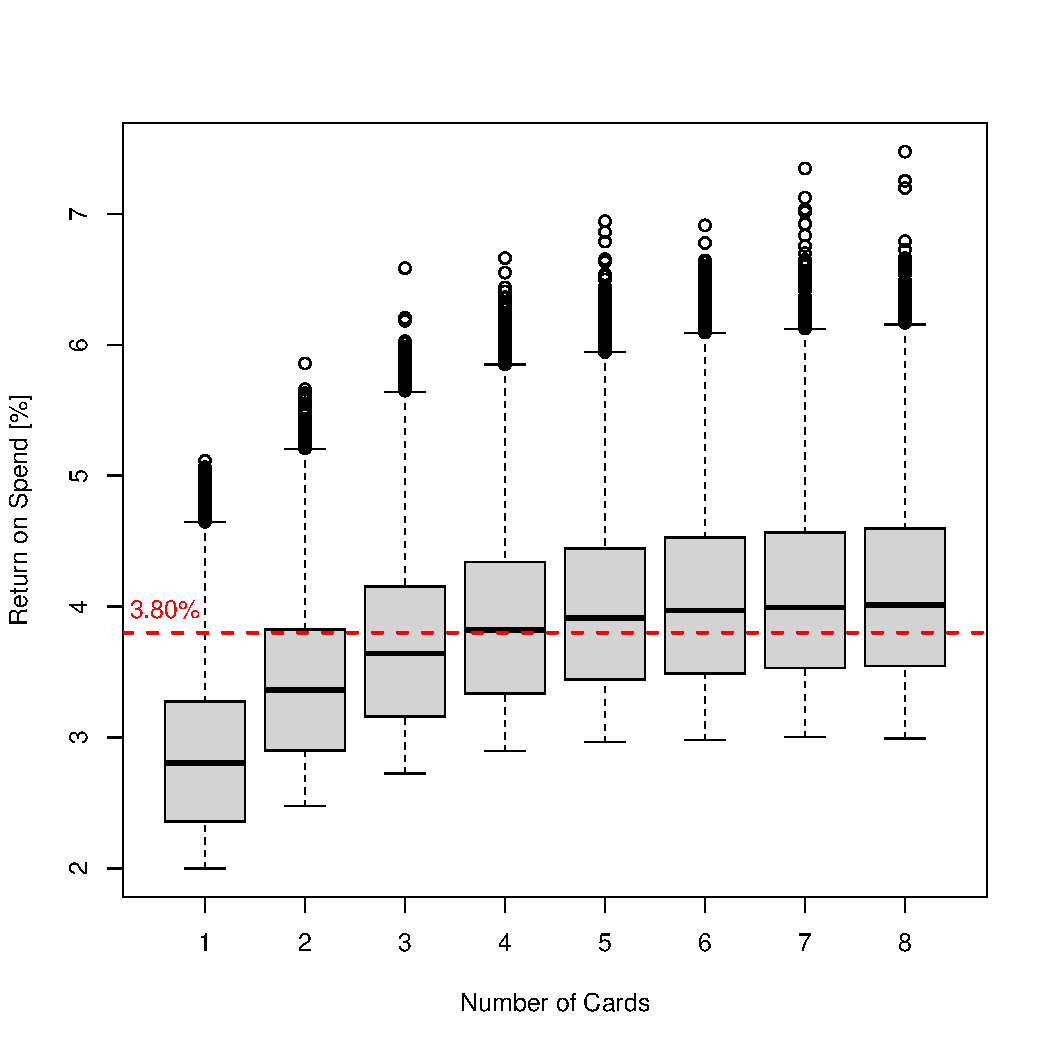
\includegraphics[width=0.9\textheight]{../Figures/MC_ROS_vs_K.pdf}
%         \end{column}
%         \begin{column}{0.3\textwidth}
%             \centering 
%         \end{column}
%     \end{columns}
% \end{frame} 

% meanlog         sdlog    
%   11.306046366    0.945677201 
%  ( 0.003960832) ( 0.002800731)
% NOTE ON LOG-NORMAL DISTRIBUTIONS FROM QUORA:
% Prices and incomes do not necessarily follow a strict log-normal distribution in practice. However, the log-normal distribution is often used to model certain economic and financial phenomena due to its mathematical properties and because it can provide a good approximation for certain types of data.

% Here are a few reasons why the log-normal distribution is sometimes used to model prices and incomes:

% Multiplicative Processes: In many economic and financial situations, changes are multiplicative rather than additive. For example, if an asset's price increases by a certain percentage each period, the overall price over time will follow a multiplicative process. The log-normal distribution is well-suited to model such multiplicative processes.
% Central Limit Theorem: The log-normal distribution can arise as a result of the Central Limit Theorem when the underlying factors influencing prices or incomes are the product of many independent random variables. In such cases, the distribution of the final outcome tends towards a log-normal distribution.
% Non-Negative Values: Prices and incomes are typically non-negative values, and the log-normal distribution is defined for positive values only. This makes the log-normal distribution a natural choice when modeling variables that cannot take negative values.
% Right Skewness: Prices and incomes often exhibit right-skewness, where there is a long tail to the right of the distribution. The log-normal distribution is characterized by a right-skewed shape, making it a plausible choice for modeling such data.
% It's important to note that while the log-normal distribution can be a convenient and useful model in certain contexts, it is not always a perfect representation of real-world data.


\section{Shiny App}

\begin{frame}
    \vfill
    \centering
    \begin{beamercolorbox}[sep=8pt,center,shadow=true,rounded=true]{title}
      \usebeamerfont{title}Demonstration!
    \end{beamercolorbox}
    \url{https://remcoscheepmaker.shinyapps.io/ReMCCO/}
    \vfill
\end{frame}

\begin{frame}{ReMCCO -- Recommend Me Credit Cards Optimally}
    \begin{center}
        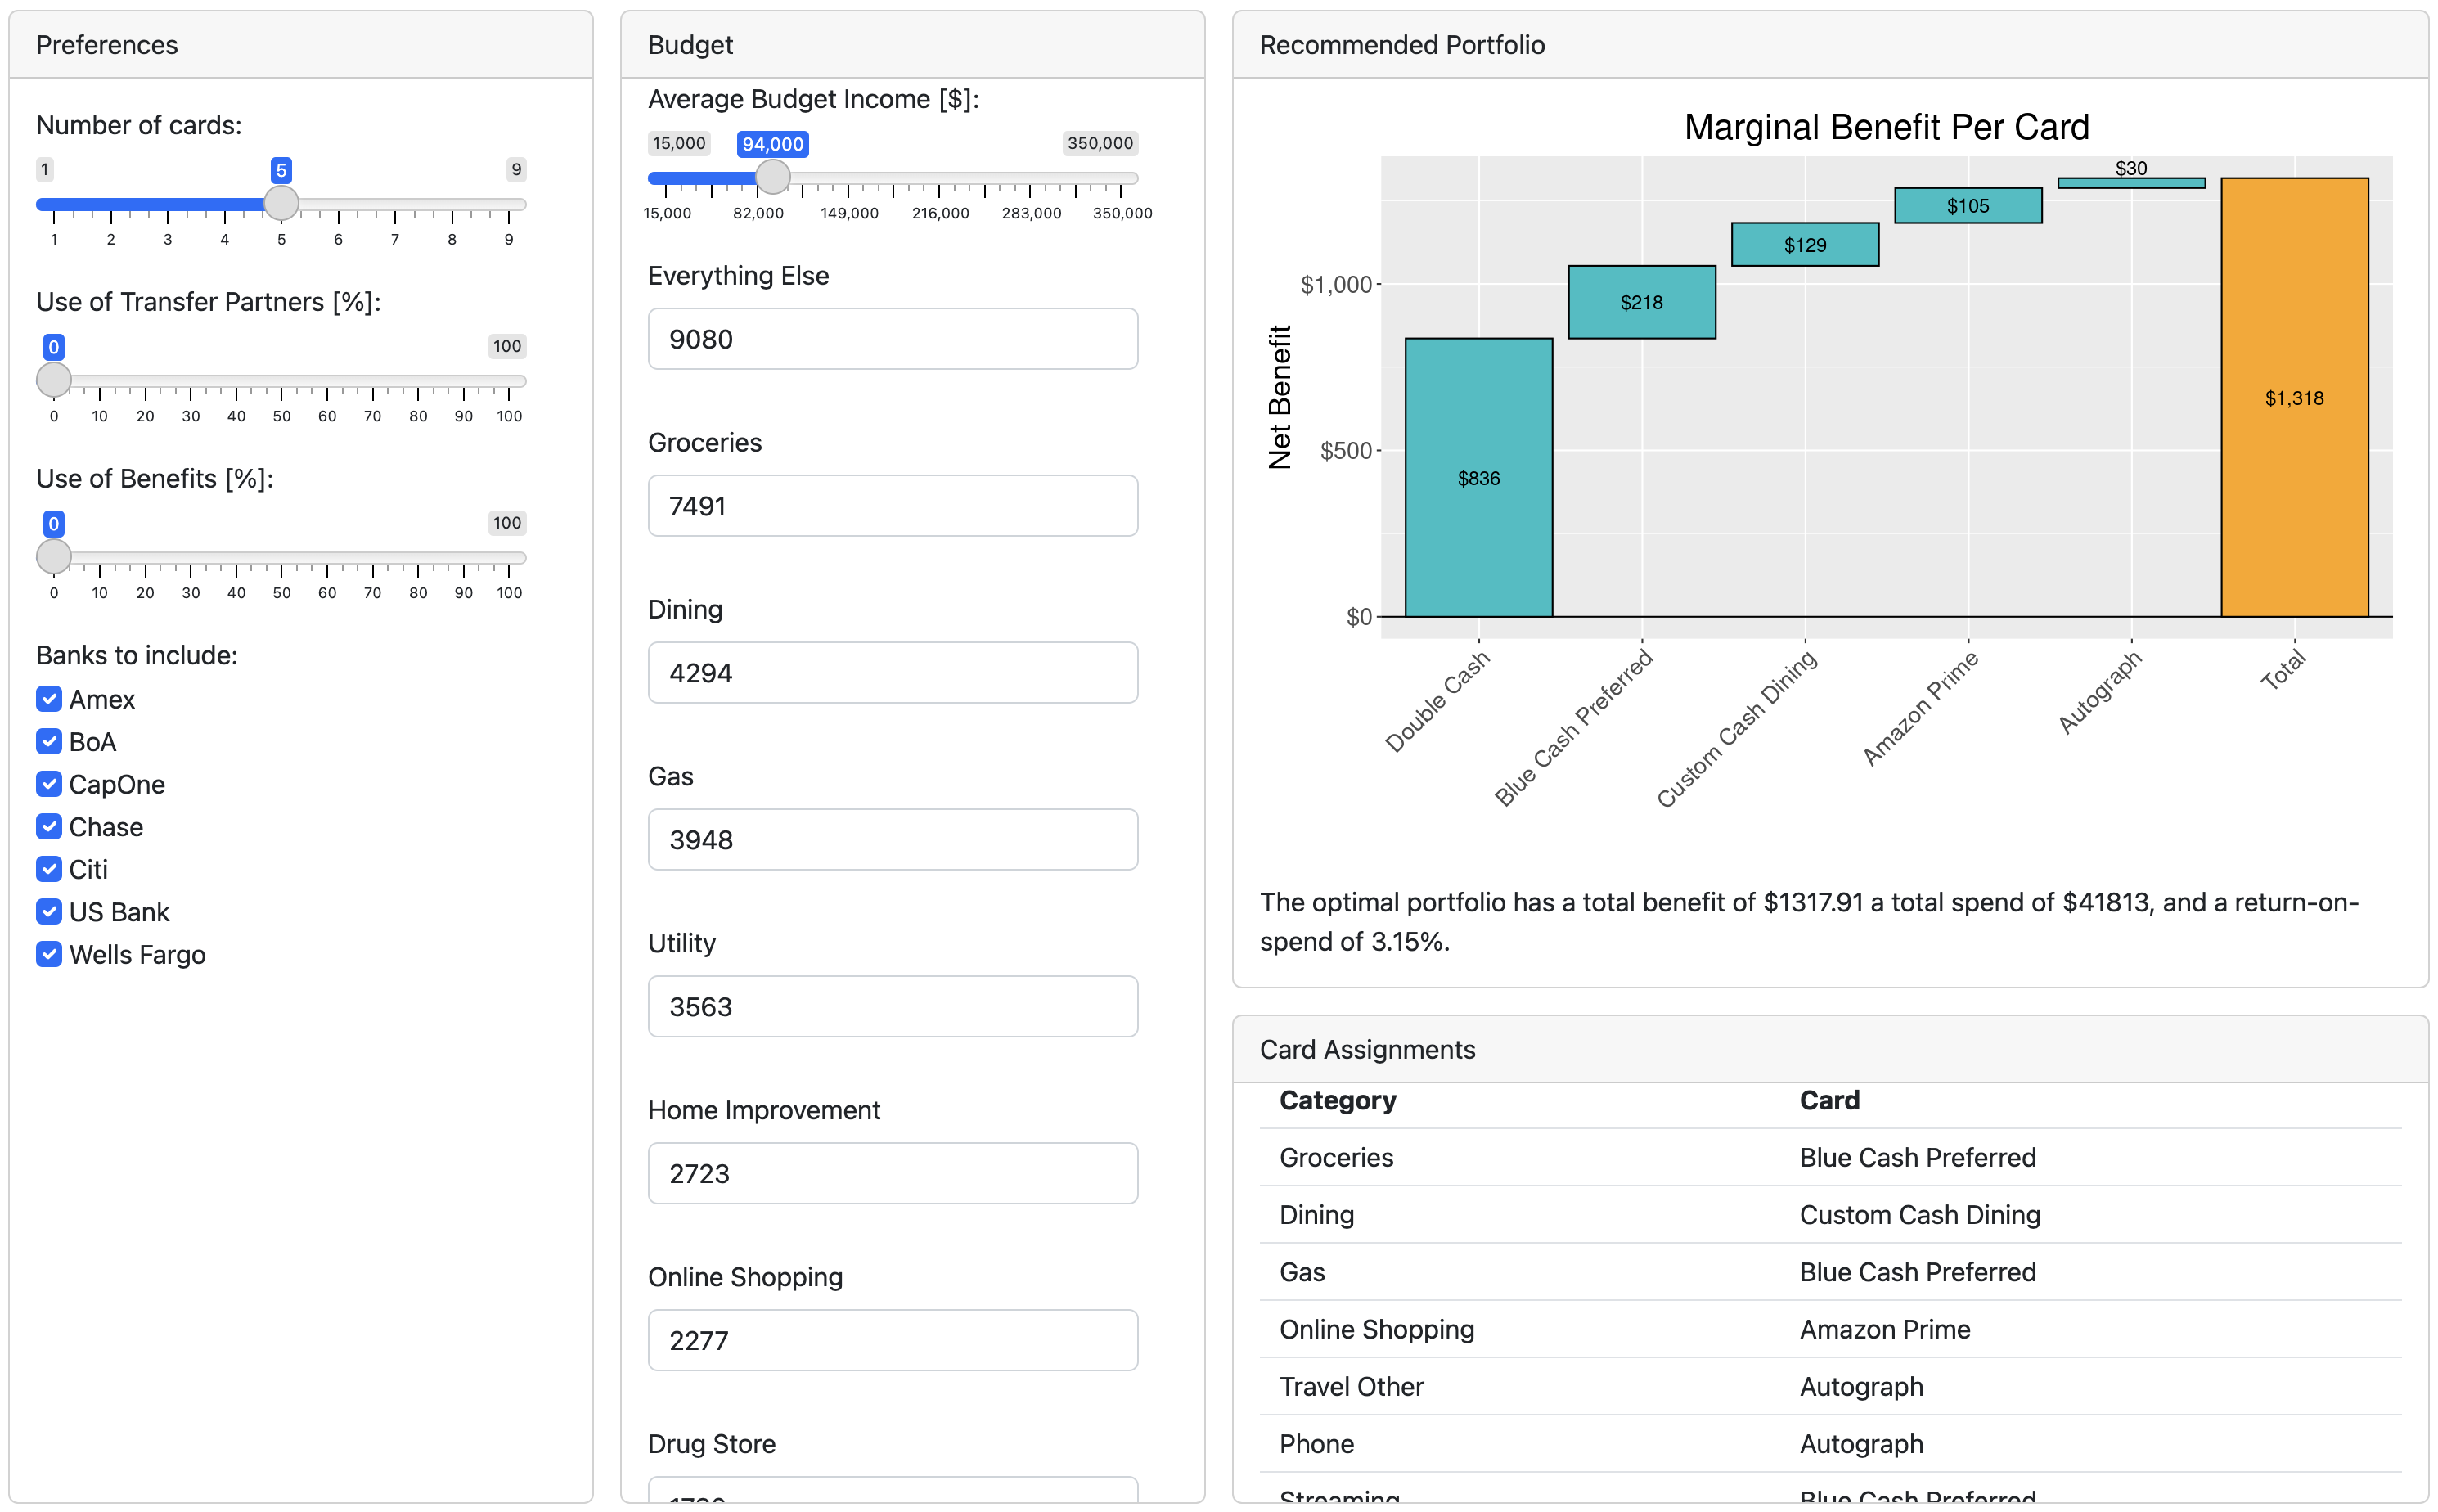
\includegraphics[width=1.0\textwidth]{../Misc/ReMCCO.png}
    \end{center}
\end{frame} 

\begin{frame}{Future Plans}
    \begin{itemize}
        \item A card recommendation app is deployed, including a bank filter and customizable budget
        \bigskip
        \item I still aim to make the following upgrades for advanced users (using hidden options or additional panels):
        \begin{itemize}
            \item Option to customize point valuations per bank
            \item Option to customize benefit valuations per travel card
            \item This will make the app more useful for Trifecta users or Bank of America Preferred Rewards members 
        \end{itemize}
        \bigskip
        \item For future scalability I'm considering moving the data to a SQL database
    \end{itemize}
\end{frame}

% Flaws
% Although the app is up and running, and there is a bank filter and custom budget, 
% I could still improve the following: 
% really want to give different value to the benefits of say Cap One vs Amex. 
% Really want to have the option to give Chase points higher value than say Cap One points,
% or say that I have Bank of America Preferred Rewards. 
%
%
% NEXT STEPS
% - Could consider making point values adjustable per bank in a tabset or a switch
% on the main panel that replaces the eta slider 
% - Same for theta: could make radio buttons to switch between slider percentage and 
% individual benefits values per premium card
% - Will try to make a database with credit card and income tables, and functions to add 
% data to the database, for future scalability.


\section{Summary \& Conclusions}

\begin{frame}
    \frametitle{Summary \& Conclusions}
    \begin{itemize}
        \item Financially sophisticated credit card users can benefit from inefficiencies in rewards programs by using the right credit cards
        \bigskip
        \item With some planning (and the use of my app), most Americans should be able to get $3.8\pm0.8$~\% back on all their spend by using 4--5 credit cards
        \bigskip
        \item Both (disciplined) low-income and high-income users benefit from credit cards disproportionally
        \begin{itemize}
            \item Low incomes could use static benefits without spending on the cards (in theory\dots)
            \item Banks stimulate travel (overspending), which benefits high incomes (who already travel) 
        \end{itemize}
    \end{itemize}
\end{frame}

\begin{frame}
    \vfill
    \centering
    \begin{beamercolorbox}[sep=8pt,center,shadow=true,rounded=true]{title}
      \usebeamerfont{title}Thank You!
    \end{beamercolorbox}
    \vfill
\end{frame}

% \section*{Appendix}

% \begin{frame}
%     \vfill
%     \centering
%     \begin{beamercolorbox}[sep=8pt,center,shadow=true,rounded=true]{title}
%       \usebeamerfont{title}Extra Slides
%     \end{beamercolorbox}
%     \vfill
% \end{frame}


% \begin{frame}{References}
%     \bibliographystyle{../chicago}
%     \bibliography{../References}
% \end{frame}    
